\chapter{Building an electronic thermometer and a thermostat}
We realized an electronic thermometer. This was achieved by using the PT100, a platinum resistor with a well known thermal coefficient $\alpha$. We made a fixed current pass through the PT100 so we had the signal represented by a voltage, then we amplified this signal and imposed through a differential amplifier the final output to be 0 V when the temperature was 0 \degree C. The aim was to have a voltage that could've easily been converted to a temperature by multipling it to a coefficient $\eta = 10 \frac{\degree C}{\text{V}}$.\\
In the last part we added to this circuit a power step, making it able to heat its surroindings and thus keeping the nearby temperature at a constant value.

\section{Materials}
\begin{itemize}
\item Operational amplifiers OP07
\item comparator LM311
\item Instrumentation amplifier (INA) AD622
\item Precision +5V Voltage Reference REF02
\item Thermoresistor PT100
\item Resistors, trimmers, capacitors
\item Transistor npn 2N2222
\item A LED
\item Power supply RIGOL DP831A
\item Waveform generator RIGOL DG1032
\item Multimeter RIGOL DM3068
\item Transistor 2N2222
\end{itemize}
All the resistors used had an uncertainty of 5\% of their nominal value.

\section{Electronic thermometer}
Firstly we measured the PT100 resistance using two different methods: one was the standard two wires measure, obtained by adding on each PT100 end two 10 $\Omega$ resistors in order to simulate the presence of parassite wire resistance. We measured $R_t \simeq 132\Omega$ which converted with $T = \frac{R_t - R_0}{R_0 \alpha}$\footnote{ $R_0$ is the PT100's resistance at 0 $\degree C$ and $\alpha$ is the thermal coefficient, that is around $0.003850 \degree C^{-1}$  }
gave us $\simeq 80\degree C$. We then used the 4 wires configuration and meausured $R_t \simeq 110 \Omega$, that means a temperaure of around $ 26 \degree C$.
\begin{figure}[H]
\centering
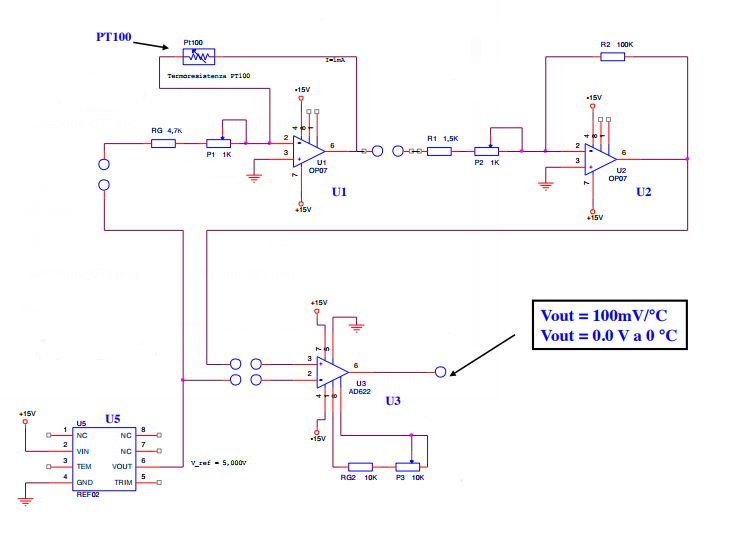
\includegraphics[width=.7\textwidth]{6/circuit.png}
\caption{full thermometer circuit}
\end{figure}
In order to build the thermometer circuit we firstly turned the resistor mesurament in a voltage mesurament: this was achieved simply making a fixed current flow into the PT100 and recording the voltage between its ends. We then needed a highly stable current generator, which means a stable input voltage: for this  reason we used the REF02 that when powered up gave an output of $4.9993 \pm 0.0003$ V. Measuring the current flowing through the PT100, we set it as close as possible to 1mA (the best value that limit self-heating) by tuning the trimmer connected to the inverting pin.\\
Since we wanted a slope of $100 \frac{mV}{\degree C}$ and given that the PT100 had a dependence from temperature of $0.3850 \frac{\Omega}{\degree C}$ with 1 mA of current flowing into it, we need to have a total gain of $G_{tot} = \frac{100 \frac{mV}{\degree C}}{0.385 \frac{mV}{\degree C}} = 259.74$.\\
We also needed to set the output to 0 mV at 0 \degree C, so we decided to first amplify the voltage on the PT100 ends by 50 times and then use this output in a differential amplifier with a gain of 5.195, where the other input should have been the voltage corresponding to $0\degree C$, i.e. 5V: this allowed us to take the first amplified signal and compare it with the reliable one from REF02.\\
In the first amplifier stage we used an OP07 in inverting configuration: its gain was set using an input voltage of 100 mV and adjusting a trimmer in order to have as output exactly 5 V.\\
In the last stage we used the AD622. Since this was the first time we worked with it we did some excercise before the connection to the circuit: we built a bridge to which we connected the AD622. We used two resistors of 100k$\Omega$ ($R_1$ and $R_2$), one of $1k\Omega$ ($R_4$) and one of $100 \Omega$ in series to a trimmer ($R_3$), we used also a resistance of 51.1 $\Omega$ (1\% of uncertainty) to set the gain of the AD622 to 1000. By changing the resistance of the trimmer we were able to nullify the output voltage.\\
\begin{figure}[H]
\centering
\begin{circuitikz}
%ponte
\draw(0,0);
\draw(0,6.7)--(0,7.2);
\node[above] at (0,7.2) {$v_{+}$};
\draw(-1,6.7)--(1,6.7);
\draw(-1,6.7)--(-1,6.2);
\draw(1,6.7)--(1,6.2);
\draw (-1,6.2) to[R,l^=$R_1$](-1,4.7);
\draw (1,6.2) to[R,l^=$R_2$](1,4.7);
\draw(-1,4.7)--(-1,3.5);
\draw(1,4.7)--(1,3.5);
\draw (-1,3.5) to[R,l^=$R_4$](-1 ,2);
\draw (1,3.5) to[vR,l^=$R_3$](1,2);
\draw(-1,2)--(-1,1.5);
\draw(1,2)--(1,1.5);
\draw(-1,1.5)--(1,1.5);
\node[sground] at (0,1.5) {};
%opamp
\draw(-1,4.69)--(4,4.69);
\draw(1,3.71)--(4,3.71);
\node[op amp] (opamp) at (5,4.2) {};
\draw(5,5.3)--(5,4.7);
\node[above] at (5,5.3) {$+v_{cc}$};
\draw(5,3.0)--(5,3.7);
\node[below] at (5,3.0) {$-v_{cc}$};
\node[right] at (6.19,4.2) {$v_{out}$};
%gain resistance
\draw(4.3,5.1)--(4.3,6.3);
\draw (4.3,6.3) to[R,l^=$R_G$](5.5,6.3);
\draw(5.5,6.3)--(5.5,4.4);
\end{circuitikz}
\caption{Testing bridge}\label{Ponte}
\end{figure}
After this test we felt confident to build a differational amplifier with a gain of 5.195 using the AD622: once put to ground the inverting pin and set a sine wave signal of 100mV to the non-inverting one, we changed the output tweaking the trimmer connected to the $R_G$ pin.\\
After the gain was brought to 5.195 we connected all the circuits together: The signal from the current generator was used as input signal in the amplifier and the output of the amplifier was placed on the non-inverting pin of the differential amplifier, while on the inverting pin was placed the voltage generated from the REF02.\\
We connected the output to the multimeter and changed the setting in order to make it show 1 \degree C to each 100mV on the screen. The value measured was around 25 \degree C and we tested that heating the PT100 caused it to increase.

\section{The P of PID}
\begin{figure}[H]
\centering
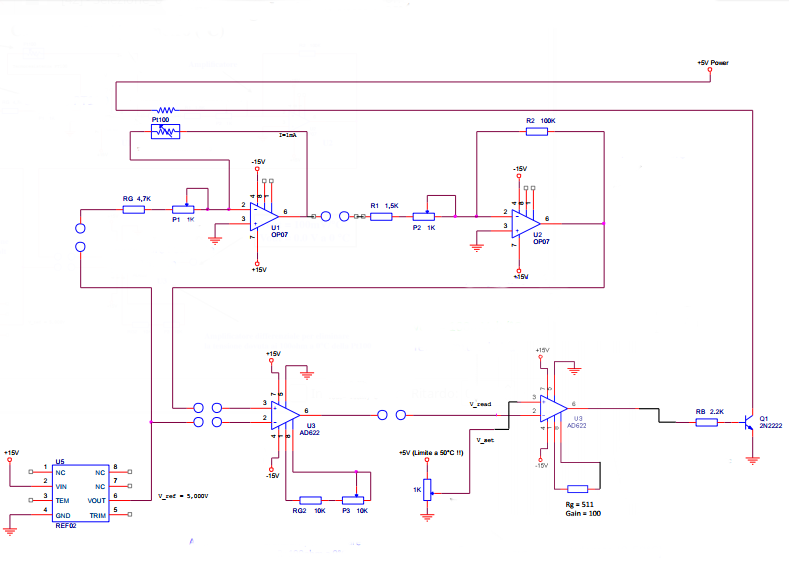
\includegraphics[width=.8\textwidth]{6/circuit2.png}
\end{figure}
We connected the thermometer output to a differential amplifier with $G=100$ in order to compare it with a reference chosen by us obtained connecting the non inverting pin to a fixed voltage through a trimmer. The INA output was connected as the base input of a NPN transistor using a resistor in between. The transitor controlled a power circuit made with a small resistence $R= 27 \Omega$ (0.5 Watt resistor) with a voltage of 5V taken from the agilent generator. The PT100 was placed next to the small resistor, measuring its temperature.\\
If the temperature set by the trimmer was different from the one measured, that difference was amplified and converted to a current flowing in the power circuit, which would heat up the resistor until the difference in temperature was nullified. The current flowing in $R$ is proportional to the temperature difference. The differential amplifier had a saturation voltage of around 10, so that the amplification of 100 allowed us to control the temperature on a range of 1 \degree C (100 mV).\\
For the current's measure we used a tester ICE placed between $R$ and the transistor. During the test, when we changed the desired temperature, we saw the current raise and then making damped oscillations towards a stable current.
